\documentclass[xcolor=dvipsnames]{beamer}

\usepackage{amsmath, amssymb, graphicx}
\usepackage[english]{babel}
\usepackage{times}
\usepackage[utf8]{inputenc}
\usepackage[T1]{fontenc}
\usepackage{listings}
\usepackage{hyperref}
\usepackage[norelsize,ruled,vlined]{algorithm2e}
\usepackage{color}
\usepackage{hyperref}
\usepackage{booktabs}
\usepackage{tikz}
\usetikzlibrary{matrix}
\usetikzlibrary{arrows}
\usetikzlibrary{positioning}
\usetikzlibrary{shapes.multipart}

\theoremstyle{definition}
\newtheorem{proposition}{Proposition}

\mode<presentation>
\usecolortheme{fly}

\setbeamercolor{alerted text}{fg=purple}

\setbeamertemplate{footline}{%
  \usebeamercolor[fg]{navigation symbols}%
  \usebeamerfont{footline}
  \parbox{\linewidth}{
    \vspace*{-8pt}
    \hspace{5pt}\insertpagenumber/\inserttotalframenumber
    %% \insertshortauthor\hspace{5pt}\insertshortinstitute
    %% \hfill \insertsection
    %% \hfill\usebeamertemplate***{navigation symbols}
    %% \hfill
  }
}
%% \setbeamertemplate{navigation symbols}{}


\title[Free Will Is Creative]{Free Will Is Creative\\
  {\small Towards A New Conception of Free Will}
}
\author{Fengyun Liu}
\institute[EPFL]{EPFL}
\date{\today}

%% set code styles

\definecolor{dkgreen}{rgb}{0,0.6,0}
\definecolor{gray}{rgb}{0.5,0.5,0.5}
\definecolor{mauve}{rgb}{0.58,0,0.82}

\lstset{
  language=scala,
  aboveskip=3mm,
  belowskip=3mm,
  showstringspaces=false,
  columns=flexible,
  basicstyle={\ttfamily\Large},
  numbers=none,
  numberstyle=\tiny\color{gray},
  keywordstyle=\color{blue},
  commentstyle=\color{dkgreen},
  stringstyle=\color{mauve},
  breaklines=true,
  breakatwhitespace=true,
  tabsize=3,
}


% Delete this, if you do not want the table of contents to pop up at
% the beginning of each subsection:
\AtBeginSection[]
{\begin{frame}<beamer>{Overview}
        \tableofcontents[
            sections={1-6},
            currentsection,
            currentsubsection,
            hideothersubsections,
            sectionstyle=show/shaded,
        subsectionstyle=show/shaded/hide]
    \end{frame}
}

\begin{document}


%%%%%%%%%%%%%%%%%%%%%%%%%%%%%%%%%%%%%%%%%%%%%%%%%%%%%%%%%%%%%%%
% 0. Titlepage
%%%%%%%%%%%%%%%%%%%%%%%%%%%%%%%%%%%%%%%%%%%%%%%%%%%%%%%%%%%%%%%
{
\setbeamertemplate{footline}{}
\begin{frame}
    \titlepage{}
\end{frame}


%% \begin{frame}{Today's agenda}
%% \tableofcontents[hideallsubsections,
%%     sections={1-6}
%% ]
%% \end{frame}
}

%%%%%%%%%%%%%%%%%%%%%%%%%%%%%%%%%%%%%%%%%%%%%%%%%%%%%%%%%%%%%%%
% 1. Background
%%%%%%%%%%%%%%%%%%%%%%%%%%%%%%%%%%%%%%%%%%%%%%%%%%%%%%%%%%%%%%%
% subsection Motivation (end)
\section{Traditional View of Free Will} % (fold)
\label{sec:Background}

\begin{frame}[fragile]
  \frametitle{Free Will as the Capacity to Choose}
  Traditional philosophers characterize free will as the \alert{capacity to choose}.

  \begin{itemize}
  \item Libertarians: \emph{The ability to do otherwise}
  \item Compatibilists: \emph{The ability to align desires and actions}
  \end{itemize}
\end{frame}

\begin{frame}[fragile]
  \frametitle{The Magic Power of Choice}
  An agent has free will can do either A or B, solely based on his/her choice.

  \begin{figure}
    \centering
    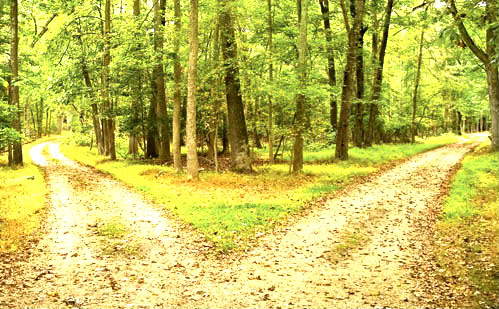
\includegraphics[width=0.8\textwidth]{images/woods.jpg}\\
    \emph{Two Roads Diverged In a Yellow Wood}
  \end{figure}
\end{frame}

\begin{frame}[fragile]
  \frametitle{The Magic Power of Choice}
  Once owned this magic power, it can be used \alert{anywhere}, \alert{anytime} and on \alert{any matters}.
  \begin{figure}
    \centering
    
\includegraphics[width=0.8\textwidth]{images/magic.jpg}\\
  \end{figure}
\end{frame}

\begin{frame}[fragile]
  \frametitle{Two Tasks of Presentation}
  I dub the view which regards \emph{free will as the magic power of choice} as the \alert{myth of choice}.\\[1cm]

  Tasks of this presentation:
  \begin{itemize}
  \item Break the \emph{myth of choice}
  \item Show that \emph{free will is creative}
  \end{itemize}
\end{frame}

%%%%%%%%%%%%%%%%%%%%%%%%%%%%%%%%%%%%%%%%%%%%%%%%%%%%%%%%%%%%%%%
% 2. The Myth of Choice
%%%%%%%%%%%%%%%%%%%%%%%%%%%%%%%%%%%%%%%%%%%%%%%%%%%%%%%%%%%%%%%
\section{The Myth of Choice} % (fold)

\begin{frame}[fragile]
  \frametitle{Free Will Is Not Irrationality}
  Rationality means you should choose the better one!

  \begin{figure}
    \centering
    
\includegraphics[width=0.8\textwidth]{images/rationality.jpg}\\
    \emph{Only an insane deliberately makes a suboptimal choice!}
  \end{figure}
\end{frame}

\begin{frame}[fragile]
  \frametitle{Rationality Is Not A Mysterious Capacity}

  \begin{lstlisting}[language=Scala]
    def decide(opt1, opt2) = {
      if (opt1 betterThan opt2)
          choose(opt1)
      else if (opt2 betterThan opt1)
          choose(opt2)
      else
          ...
    }
  \end{lstlisting}
\end{frame}

\begin{frame}[fragile]
  \frametitle{Free Will Is Not Hesitation}
  If A and B are seemingly equally good, then you're in trouble!

  \begin{figure}
    \centering
    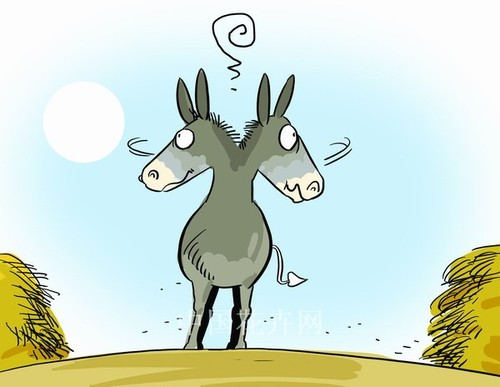
\includegraphics[width=0.8\textwidth]{images/ass.jpg}\\
    \emph{Buridan's ass}
  \end{figure}
\end{frame}

\begin{frame}[fragile]
  \frametitle{Free Will Is Not Hesitation}
  Two seemingly equally good choices may not be equal in fact, it's only that you are unable to differentiate them.\\[0.5cm]

  Hesitation is usually a reflection of \alert{inability} to decide efficiently, where you need help from experts -- more experienced and informed people in the field, or you need more training in the field.
\end{frame}

\begin{frame}[fragile]
  \frametitle{Hesitation Is Not A Mysterious Capacity}

  \begin{lstlisting}[language=Scala]
    def decide(opt1, opt2) = {
      if (opt1 betterThan opt2)
          choose(opt1)
      else if (opt2 betterThan opt1)
          choose(opt2)
      else
          decide(opt2, opt1)
    }
  \end{lstlisting}
\end{frame}

\begin{frame}[fragile]
  \frametitle{Free Will Is Not Randomness}
  If you resort to randomness, you are giving up free will!

  \begin{figure}
    \centering
    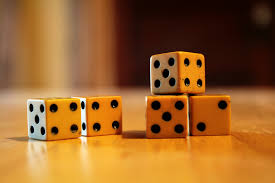
\includegraphics[width=0.8\textwidth]{images/dice.jpg}\\
  \end{figure}
\end{frame}

\begin{frame}[fragile]
  \frametitle{Free Will Is Not Randomness}
  Resorting to randomness to try luck implies you are aware that the two choices are very likely to be unequal, but unable to differentiate them.\\[0.3cm]

  Failure to differentiate the better choice and resorting to randomness \alert{unnecessarily} is a reflection of \alert{inability}.\\[0.3cm]

  Resorting to randomness doesn't mean some real random process in the world, it only means you let yourself to be determined by external forces that you can't predict.
\end{frame}


\begin{frame}[fragile]
  \frametitle{Randomness Is Not A Mysterious Capacity}

  \begin{lstlisting}[language=Scala]
  def decide(opt1, opt2) = {
    if (opt1 betterThan opt2)
       choose(opt1)
    else if (opt2 betterThan opt1)
       choose(opt2)
    else
       choose(random(opt1, opt2))
  }
  \end{lstlisting}
\end{frame}

\begin{frame}[fragile]
  \frametitle{Free Will Is Not the Capacity to Decide}

  The \alert{myth of choice} bankrupts:
  \begin{itemize}
  \item The capacity to decide can't differ from the program
  \item There's nothing special about the capacity to decide
  \item The capacity to decide can't honor the name \emph{free will}
  \end{itemize}
\end{frame}


%%%%%%%%%%%%%%%%%%%%%%%%%%%%%%%%%%%%%%%%%%%%%%%%%%%%%%%%%%%%%%%
% 3. Free Will is Creative
%%%%%%%%%%%%%%%%%%%%%%%%%%%%%%%%%%%%%%%%%%%%%%%%%%%%%%%%%%%%%%%
\section{Free Will is Creative} % (fold)
\label{sec:creative}

\begin{frame}[fragile]
  \frametitle{Free Will is Creative}

  If we exclude the \alert{capacity to decide} from free will, the only thing left that can honor free will is \alert{the capacity to generate choices}.
\end{frame}

\begin{frame}[fragile]
  \frametitle{Free Will is Creative}

  More creative one is, better choices can be generated and decided, thus more free one is.

  \begin{figure}
    \centering
    
\includegraphics[width=0.8\textwidth]{images/creativity.jpg}\\
  \end{figure}
\end{frame}

\begin{frame}[fragile]
  \frametitle{Free Will Varies in Degrees}

  Creativity varies in degrees, thus free will \alert{varies in degrees}.\\[0.5cm]

  One's free will improves if one's creativity improves.
\end{frame}

\begin{frame}[fragile]
  \frametitle{Free Will is Thematic}

  Creativity is thematic, thus free will is also \alert{thematic}.\\[0.5cm]

  The correct grammar for talking about free will is: \alert{X exhibits free will on topic T}.
\end{frame}

\begin{frame}[fragile]
  \frametitle{Creativity Honors Free Will}

  Human beings can still be proud of their free will, as they are much more creative on a lot of more topics than animals.

  \begin{figure}
    \centering
    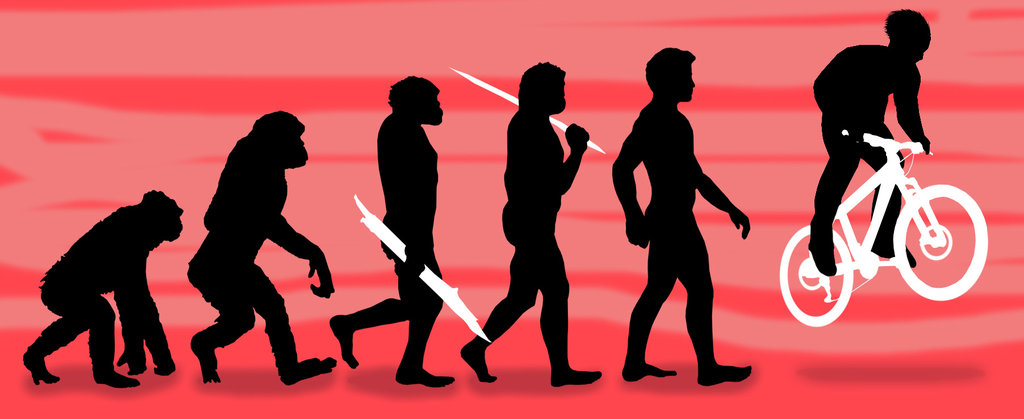
\includegraphics[width=1\textwidth]{images/degrees.jpg}
  \end{figure}
\end{frame}



%%%%%%%%%%%%%%%%%%%%%%%%%%%%%%%%%%%%%%%%%%%%%%%%%%%%%%%%%%%%%%%
% 4. Conclustion
%%%%%%%%%%%%%%%%%%%%%%%%%%%%%%%%%%%%%%%%%%%%%%%%%%%%%%%%%%%%%%%
\section{Conclusion} % (fold)
\label{sec:conclusion}

\begin{frame}[fragile]
  \frametitle{Conclusion}

  Free will is NOT the \alert{capacity to decide}:
  \begin{itemize}
  \item Free will is not irrationality
  \item Free will is not hesitation
  \item Free will is not randomness
  \end{itemize}\\[0.6cm]

  Free will is the \alert{capacity to generate choices}:
  \begin{itemize}
  \item Free will is creative
  \item Free will is rational
  \item Free will is thematic
  \item Free will varies in degrees
  \end{itemize}
\end{frame}

\begin{frame}[fragile]
  \frametitle{Question and Answers}

  \begin{center}
    \Huge{Thank you!}
  \end{center}

\end{frame}

\end{document}
